
\chapter{Design}
\label{CH-Design}

\section{Overall Concept}

The design goals for the labview architecture are as follows:

\begin{enumerate}
  \item{Improved fault tolerance}
  \item{Improved data quality \& collection uptime}
  \item{Algoritm isolation for testing and run-time stability}
  \item{Expandable}
  \item{Flexibility to accommodate hardware configuration changes}  \item{Intuitive to new users}
\end{enumerate}

To accomplish these goals, the following concept is proposed. Small individual programs (children) are written to control conceptually seperate processes which interact with the WV DIAL hardware in various ways. In general no more than one child will interact with one piece of hardware to ensure that hardware faults are isolated. These children can run in parallel with proper synchronization and communication via their queues. If one child needs to talk to another it can open that child's queue and add an element onto it. A main container is used to call collections of children programs to accomplish various tasks, and open the necessary children automatically. These sub-functions are all called by the main function based on configure files that correspond to buttons on the main panel. The operational setups that are called by the main function are:

\begin{enumerate}
\item{Warm up sub-function that brings all hardware to operational status. This includes things like warming the lasers and warming the etalons, which needs to be done before high quality data can be taken.}
\item{Main operations sub-function that performs all the mission critical hardware communication during data collection.}
\item{A template sub function which brings up an empty child with minimal functionality.}
\item{Switches sub-function which tests our ability to control the switches.}
\item{Temp. Scan sub-function which sweeps through temperatures to test the lasers.}
\item{Testing sub-functions for individusal controls to check operational status of hardware pieces such as the wavemeter (laser locking), the MCS operation, or the weather station.}
\end{enumerate}

This creates a 3 tiered structure: 1) Main function that opens sub-functions, 2) sub-functions that organize and manage children, and 3) children that actually set and control the state of each individual hardware piece. This creates a natural hierarchy that is predefined. New users unfamiliar with the operation of WV DIAL do not need to know how to control each piece individually but rather are guided through operation. Testing new hardware does not require complete integration with an all in one solution like is currently available, but can be built and tested independantly of the operations of the rest of the DIAL unit. This isolation creates fault tolerance because if one child fails, others are not waiting on that task and data collection for other children can continue unimpeded. Finally, knowledge of the hardware configuration is only needed at the higher levels (the main function and sub-functions) and can be more easily defined than a single all in one program. 

\section{Individual Element Controls}
The proposed software update parses the main hardware control function into sub-functions. The sub-functions for individual controls are:

\begin{enumerate}
\item{MCS}
\item{Weather Station}
\item{Laser Locking}
\item{Housekeeping}
\item{UPS}
\item{HSRL Oven}
\item{Wavemeter}
\item{Thor 8000}
\item{Quantum Composer}
\item{Power Switches}
\item{NetCDF}
\end{enumerate}

\subsection{MCS}\label{Sec:MCSSubFunction}

A sub-function that brings up two children. One does the communications via UDP to read the MCS, while the other is a set of controls to change the state of the MCS. These were split into two functions in order to prioritize the UDP communication so photon counting data was always running without interuption, and so that while the child was reading the UDP port the controls would continue to feel responsive. In a previous version of the MCS software putting the UDP communications in the same VI as the controls would lead to delays in the responsivness of the front panel due to the translation from a series of controls into a 32 bit hex word and back that was needed for MCS communications. 

\subsection{Weather Station}\label{Sec:WSSubFunction}

A sub-function that brings up the weather station child to monitor surface level temperature, pressure, relative humidity, and absolute humidity. 

\subsection{Laser Locking}\label{Sec:LLSubFunction}

A sub-function that brings up the laser locking routines that controls laser wavelengths and the etalons. 

\subsection{Housekeeping}\label{Sec:HousekeepingSubFunction}

A sub-function that brings up one child whose responsibility is to relay information about the temperature of the container. Thermocouples are placed within the container in various positions (which can be specified for writing into the data in the Configure\_WVDIALPythonNetCDFHeader.txt) primarily to help ensure that the climate control for the unit is functioning properly. 

\subsection{UPS}\label{Sec:UPSSubFunction}

A sub-function that calls the UPS child to monitor the state of the UPS Battery and power to the unit. 

\subsection{HSRL Oven}\label{Sec:HSRLOvenSubFunction}

A sub-function that ....

\subsection{Wavemeter}\label{Sec:WavemeterSubFunction}

A sub-function that ....

\subsection{Thor 8000}\label{Sec:T8000SubFunction}

A sub-function that ....

\subsection{Quantum Composer}\label{Sec:QCSubFunction}

A sub-function that ....

\subsection{Power Switches}\label{Sec:PowSwitchSubFunction}

A sub-function that ....

\subsection{NetCDF}\label{Sec:NetCDFSubFunction}

A sub-function that ....



\section{Back Panel Design}\label{Sec:BPDesign}

A template was made to standardize all labview control for WV DIAL. The design is to use queues to execute commands. This allows for an intentional bottleneck of execution such that user and automatically generated commands can not be executed out of order and there are a minimum of changes that need to be made to accommodate new hardware. The automatically generated and user generated commands are in the form of a string that is delimitated by an ``\_". The main loop cases are:
\begin{enumerate}
\item{Configure}
\begin{enumerate}
\item{Reads default state out of the configure file}
\item{Sets the value of all available controls per the configure file}
\item{Sets the function visibility based on control settings like RunAsChild and permissions settings}
\end{enumerate}
\item{Initialize}
\begin{enumerate}
\item{Communicate the initial state of the labview controls to the hardware or vice versa as appropriate}
\item{Create needed file folders for data saving}
\end{enumerate}
\item{Idle}
\begin{enumerate}
\item{Performs baseline commands needed to keep program running}
\item{Waits for user commands to change the state of the system}
\item{Allows for raw data visualization as appropriate}
\end{enumerate}
\item{Error Handler}
\begin{enumerate}
\item{Records all errors in an error log for debugging}
\item{Attempts recovery procedure if the error is recognized}
\item{Alerts the user if error are time sensitive and/or mission critical}
\end{enumerate}
\item{Commanded Exit}
\begin{enumerate}
\item{Performs necessary steps to shutdown hardware that are specific to being told to shut down (only accessible in RunAsChild mode)}
\end{enumerate}
\item{Exit}
\begin{enumerate}
\item{Performs necessary steps to shutdown hardware that are general to RunAsChild or not}
\item{Makes all hidden variables visible again for coding}
\end{enumerate}
\end{enumerate}


\begin{figure}[!h]\centering
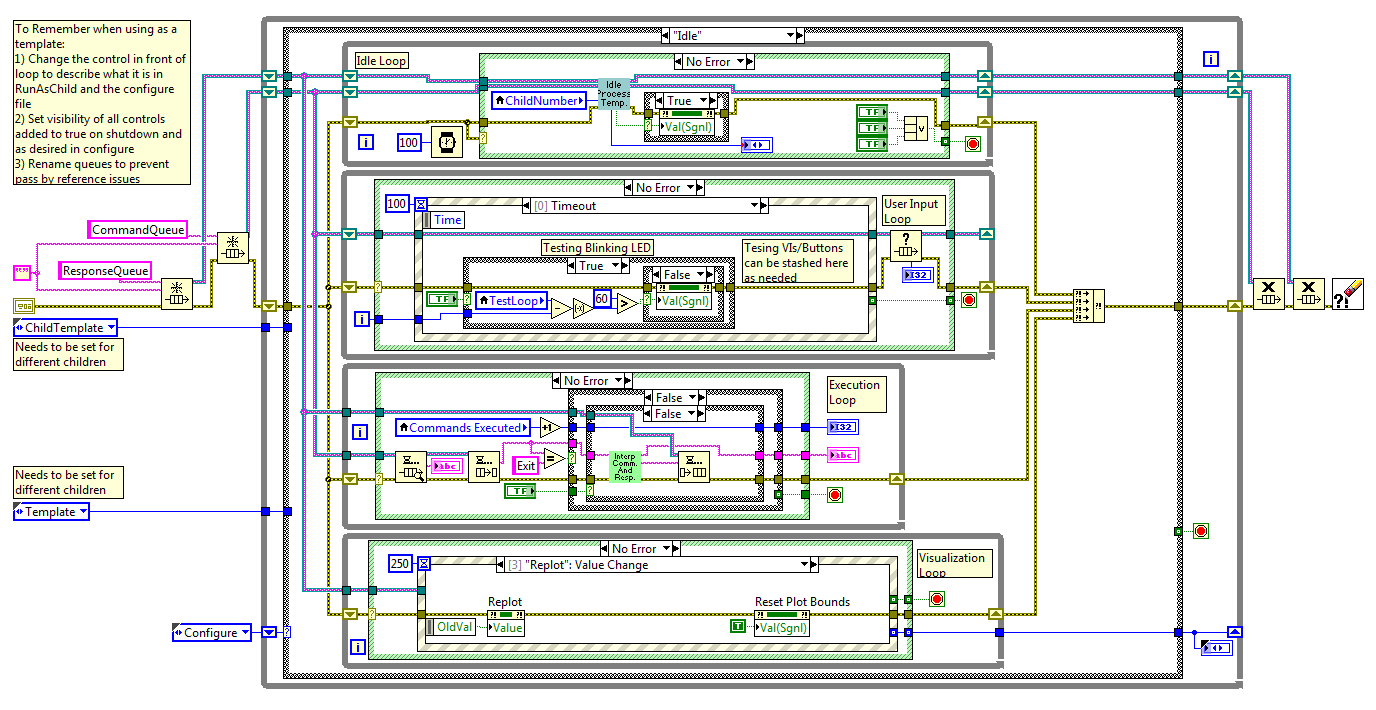
\includegraphics[height=3in]{Figures/MainVITemplateBackPanel}
\caption{A picture of the idle loop stage of the VI template child.}
\label{Fig:VITemplateBP}
\end{figure}

\subsection{The Command and Response Queues}

We have two queues, Command and Response. The command queue is meant to hold user inputs and to process those serially, changing the state of operations. The response queue is meant to hold final data products meant to be written to disk and/or displayed to the screen. The names of these queues is very important. If two queues are running in seperate children with the same name both children will be attempting to put information onto the queues and removing information off of the queues at the same time. When unintended this will cause significant problems in operations. However, this behaviour can be used to facilitate communications between children without the use of global variables and is used to elimiate race conditions that global variables can have. The most prominent example of this usage is with the queue for advanced visualization which is called by different children to communicate the nessicary information to compute and display derived fields.  

\subsection{The Idle Loop}

In the idle loop shown in Figure~\ref{Fig:VITemplateBP}, 4 while loops run. The idle loop is executing commands that are needed to maintain communication with the main function and is used to automatically control the hardware. The user input loop is waiting for user commands and adding them to the command queue. The execution loop is processing elements off of the command queue and taking action within the Interpret Commands and Responses subVI. Critically, this function is called in re-entrant execution mode as it is copied in all functions. Lastly the visualization loop which is used to process hardware responses from the response queue, save the results to disk, and to print the results to the screen. 

\subsection{Run as Stand Alone}

The multiple function concept requires one functional distinction. One concept is to run each piece manually, and another is to have a main function run each piece automatically, refered to as running in stand alone mode or running as child, respectively.   

A template for the individual control elements is given in Figure \ref{Fig:VITemplate}. There are 3 main boxes, the first is in the top left (labeled as ``Place Commands Here") for all of the user controls and everything the user needs to see. This will be different for each control. Within that box is a smaller box that would be the same for all controls that help locate the current status of the queue. The second box directly below would appear if the control were running as a stand alone but be hidden if the control were running as child. This really only needs to be in one place and is constant for all functions. The final box to the right is always hidden but is the storage place for all hidden variables that need to be defined but that the user does not need to see. 

\begin{figure}[!h]\centering
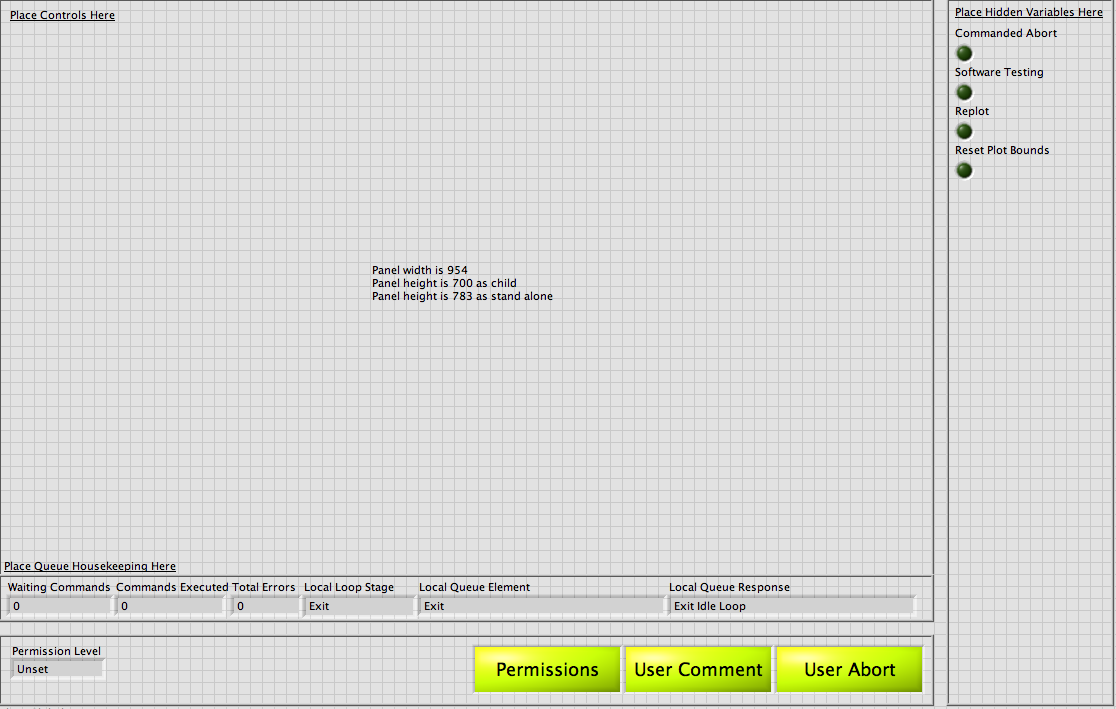
\includegraphics[height=3in]{Figures/MainVITemplate}
\caption{The front panel of the main VI template. The software at runtime will hide the unnecessary controls and shrink the front panel window the the appropriate size indicated by the outer boxes. If the VI is run as a child (called from a higher VI) the Global Buttons disappear. }\label{Fig:VITemplate}
\end{figure}

This standardization is not critical for running all VIs as stand alone, however, the solution for running all the VIs as children in parallel does. 

\subsection{Run as Child}

For the case that these individual controls are to be run automatically in parallel, an organizational problem arises. Assuming the code running the individual controls as children knows what functions to open and in what order, it is still possible that a user accidentally closes one function or a mess of VIs appears. To solve this, all front panels of the VIs running are projected into a single container seperated by a tabular control. The container itself has very little code running but is just there to contain all of the sub-VIs. This container is shown in Figure \ref{Fig:VIContainer}.

\begin{figure}[!h]\centering
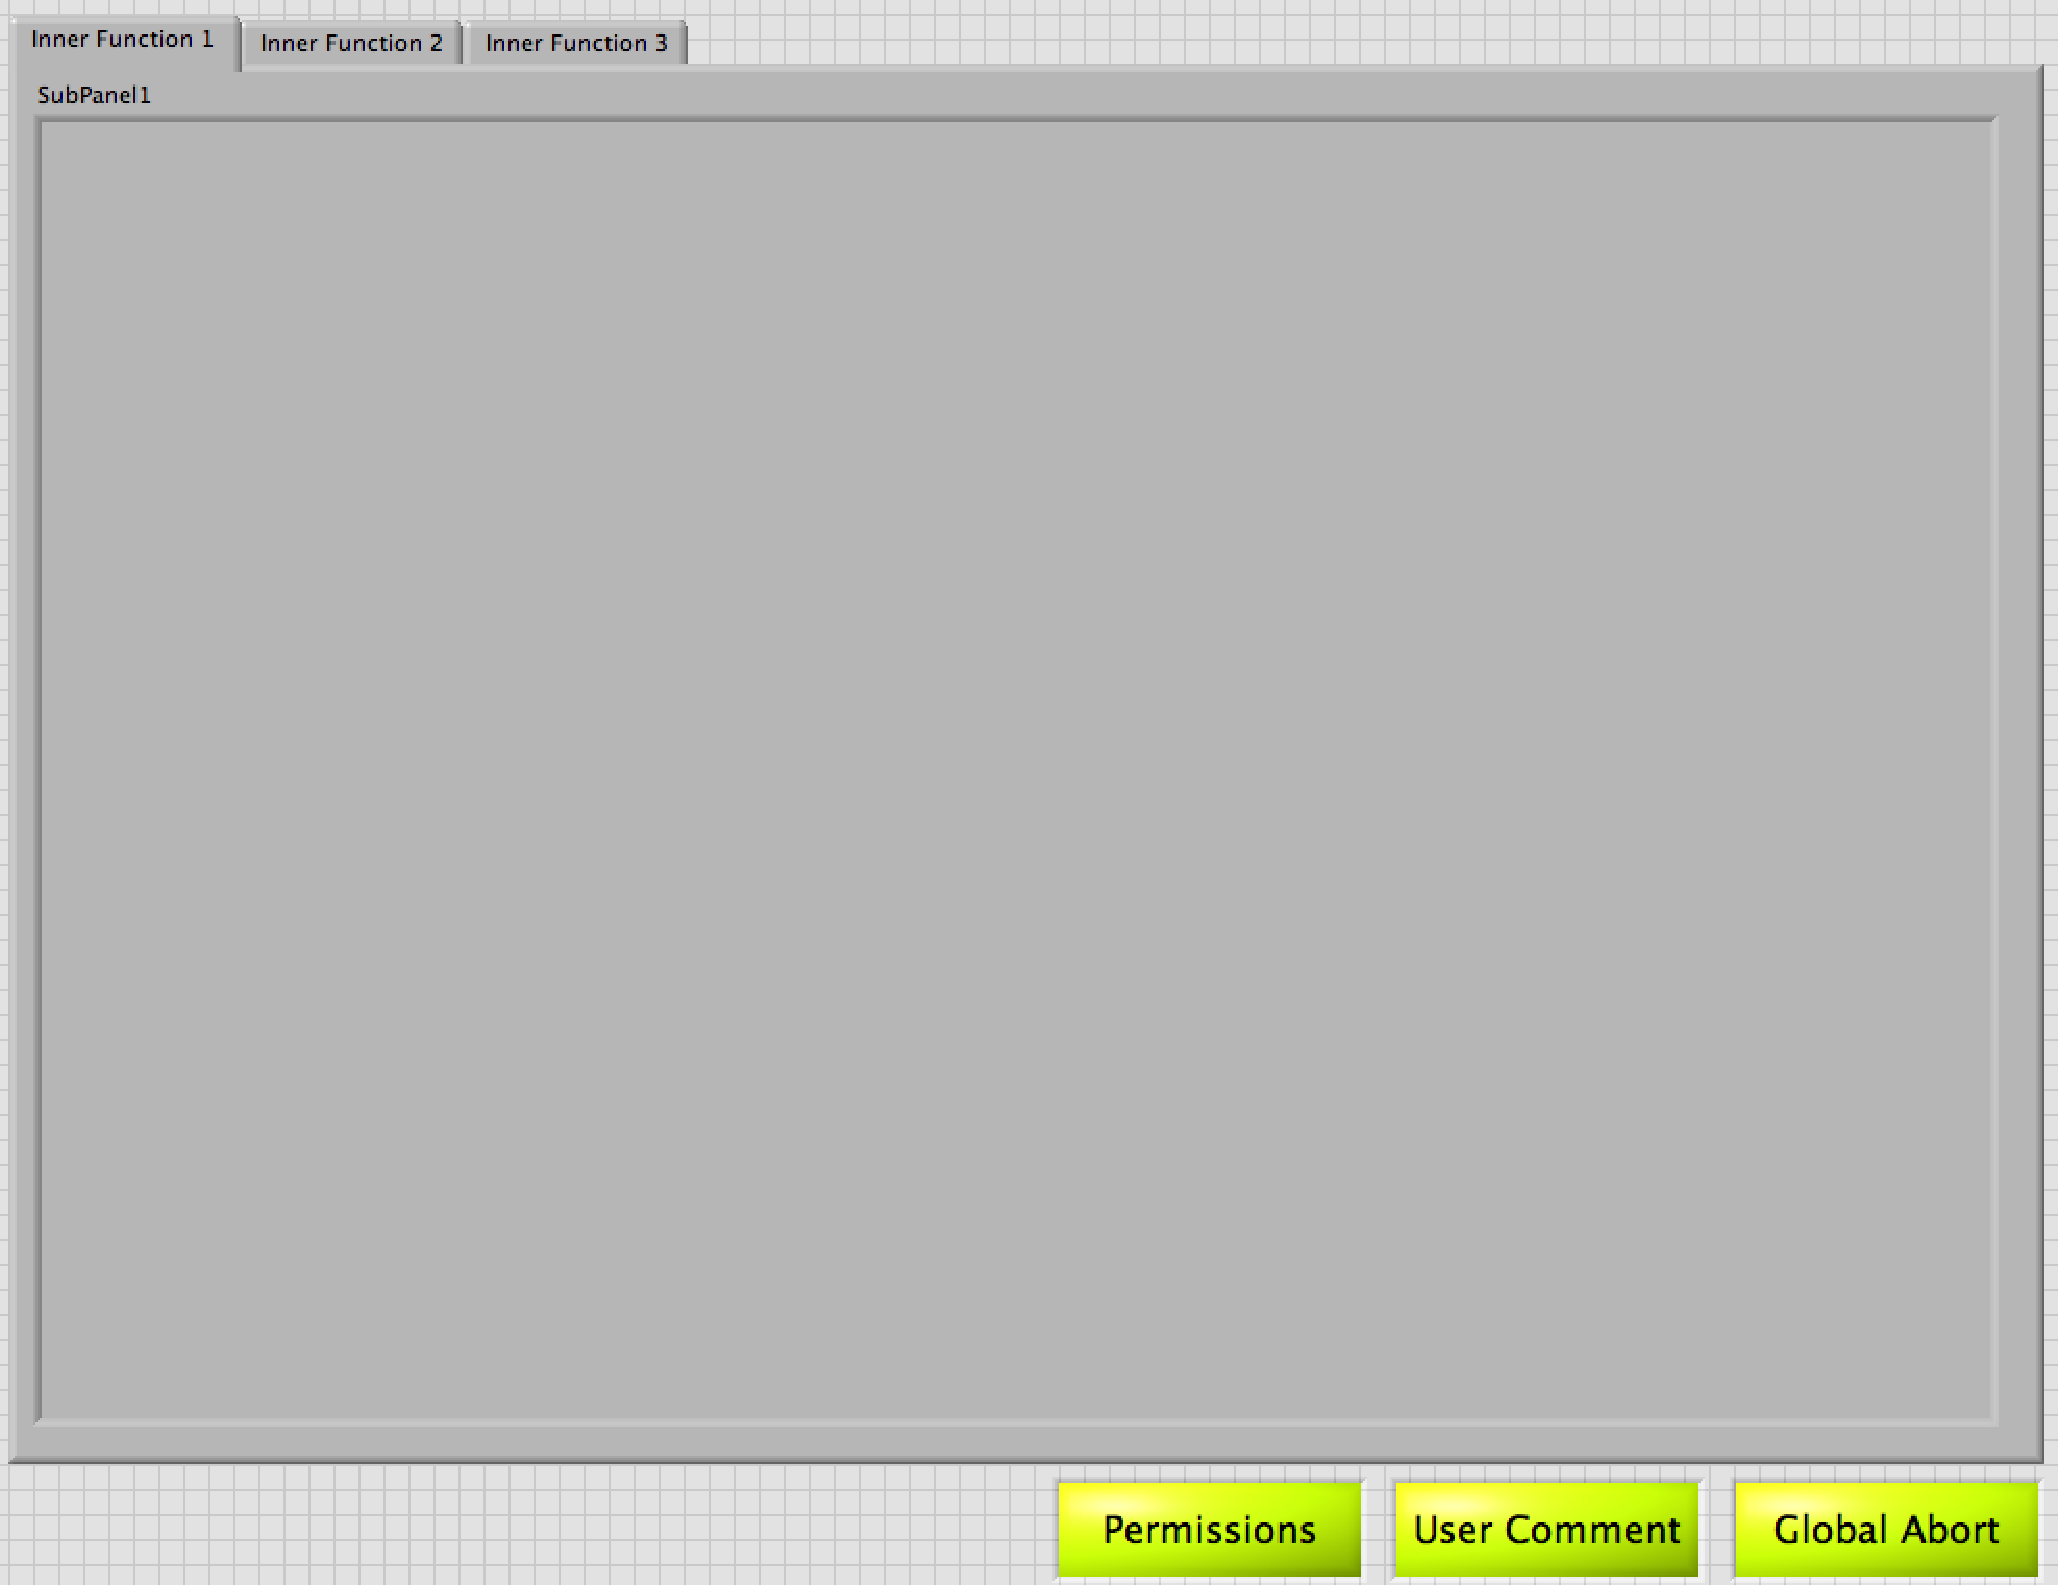
\includegraphics[height=3in]{Figures/MainVIContainer}
\caption{The front panel of the main VI container. If multiple VIs are called and run simultaneously, their front panels are projected into the main container to allow for a simple control for the user but also allows maximum flexibility in VI execution.}\label{Fig:VIContainer}
\end{figure}

In this case, the controls that are common to all VIs, in the bottom box of Figure \ref{Fig:VITemplate}, are collected and included only once. Because the front panels of all VIs are to be projected into a single container, the front panel sizes of all VIs should be of a standard size otherwise the container would not simplify much. The container itself  is simply a set of sub-panels that can each hold a single VI. The maximum number of VIs needed can be written if fewer are required, and the main program simply hides unused sub-panels. 

\subsection{Configure Files}
Instead of using default variables in Labview, the default configuration for each sub-program will be stored in a configuration file. This ensures that operational hardware configurations are decoupled from any software upgrades or changes. Additionally, it makes it always possible to return the software to a known pre-set operational state and makes it more difficult for users to unknowingly modify the hardware's initial state. The configure files are version controlled via Git to track changes over time. An example of a configure file is given in Figure \ref{Fig:ConfigureFile}. 

\begin{figure}[!h]\centering
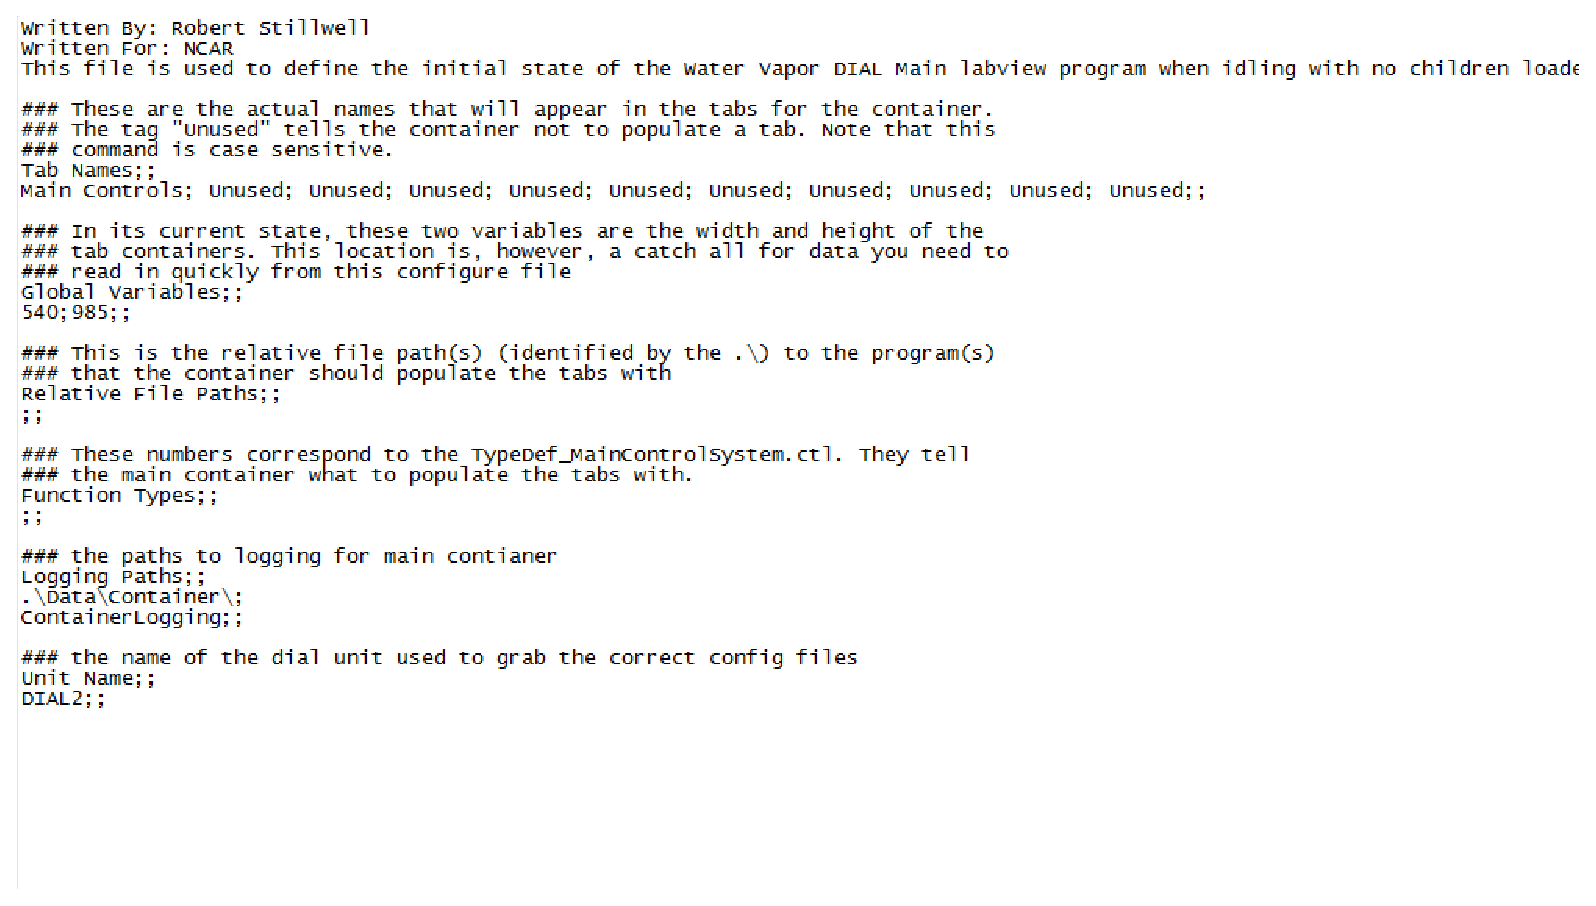
\includegraphics[height=3in]{Figures/ConfigureFileExample}
\caption{An example of the structure of a configure file. Variables are identified by a single name followed by two semi-colons. The next line has the required values delimitated by a single semi-colon with the end of line denoted by a double semi-colon.}\label{Fig:ConfigureFile}
\end{figure}

\subsection{Log Files}

Log files are to be kept to help track the status of WV DIAL and to help debug any anomalous states. The logs to be kept are:

\begin{enumerate}
\item{Operations Logs: Describes when the system starts and stops and any user defined changes}
\item{Warning logs: These indicate failures in operations which does not inhibit mission critical functionality.}
\item{Error logs: These indicate failures in mission ciritical functionality and must be addressed imediatly.}
\end{enumerate}

\subsection{Type Definitions}

One of the unfortunate features of labview occurs when trying to modify the contents of a complicated structure. For example, if you initially make a cluster to define the state of a single laser and wish to add a piece to that structure, labview will show each connected wire as broken throughout the entire program. To solve this, labview allows the user to define structure types and to link the controls on all panels directly to that definition. This allows the user to make a change in a single place and have all variables referenced to that place change at the same time. 

This type definition is widely used for controls. It requires an extra step to make the definition then load it into the program much like defining a global variable but it makes updating and maintaining the code simpler and cleaner. 

\section{Sub-Functions and Calling}

All of the individual controls are collected into a single container to run more complicated tasks. For example, the main operation of WV DIAL at full capability would require simultaneous control of the MCS, weather station, laser locking, etc.... The labview code would simply run the 6 individual controls responsible for each of these tasks and store them in a single container. 

If a single VI fails, the other sub-functions are not affected by it. Its data would be missing from the global data however. For example, if the weather station communication failed, that data would be missing but it is not completely critical to have at all times. When its service could be restored, its data stream would be restored without interuption of other services. Details of how that data appears is outlined in Chapter~\ref{CH-DATA}.

\newpage 
